\documentclass[a4paper,twoside,final]{article}
%----Eingebundene Bibliotheken-----
\usepackage[ngerman]{babel}         % Deutsches Sprachpaket
\usepackage[utf8]{inputenc}         % Eingaben codieren
\usepackage[T1]{fontenc}            % Umlaute codieren, Silbentrennung
\usepackage{amsmath, amssymb}       % Mathe
\usepackage{amsthm,amstext,amsxtra} % Symbole für Mathe
\usepackage{mathtools}              % \Aboxed Boxen in align
\usepackage{wrapfig}                % Bilder umfließen
\usepackage{svg}                    % Vektorgraphiken einbinden
\usepackage{geometry}               % Papierformat
\usepackage{tabularx}               % Tabellen
\usepackage{xcolor,colortbl}        % Farben
\usepackage{graphicx}               % Für Limes Definition wichtig
\usepackage{soul}                   % Unterstreichungen
\usepackage[section]{placeins}      % \Floatbarrier
\usepackage{wrapfig}                % Bilder umfließen
\usepackage{enumerate}              % Aufzählungen
\usepackage{footnote}               % Fußzeilen
\usepackage{booktabs}               % publication quality tables
\usepackage[hyphens]{url}           % \url{}
\usepackage{bm}                     % bold symbols \bm{r}
\usepackage{dsfont}                 % identity matrix \mathds{1}
\usepackage{enumitem}               % itemize Umgebungen customizen
\usepackage{esint}                  % Doppelintegrale
\usepackage{fancyhdr}               % schöne Kopf- und Fußzeilen
\usepackage{lmodern}
\usepackage{tikz}
\usepackage{pgfmath, pgfplots}
\usepackage[labelfont=bf]{subcaption}
\usepackage[square,numbers,sort&compress]{natbib}
\usepackage{mhchem}                 % Chemistry Package
\usepackage{physics}
\usepackage{chemfig}
\usepackage[detect-all,
            locale=DE,binary-units,
            exponent-product=\cdot
            ]{siunitx}              % \SI{12}{\gram}
%siunitx stellt für Tabellen den Spaltentyp S bereit ==> Ausrichtung an Dezimaltrennzeichen
\usepackage[position=below,
            tableposition=top,
            format=hang,
            labelfont=it,
            labelfont=bf,
            ]{caption}              % Settings für Captions
\captionsetup[wrapfigure]{name=Abb.}
\usepackage[europeanvoltages,
            europeancurrents,
            europeanresistors,
            americaninductors,
            europeanports
            ]{circuitikz}           % Schaltungen
\usepackage{chngcntr}               % vor hyperref laden!
  \counterwithin*{equation}{section}
  \counterwithin*{figure}{section}
  \counterwithin*{table}{section}

\usepackage[final,
            pdfauthor={Martin Beyer, Vanessa Huth},
            pdfsubject={Fortgeschrittenen-Praktikum},
            pdffitwindow=true,      % resize document window
            pdftitle={Fortgeschrittenen-Praktikum},
            bookmarks=true,         % lesezeichen-Liste
            bookmarksopen=true,     % Lesezeichen geöffnet
            bookmarksopenlevel=1,
            bookmarksnumbered=true,
            colorlinks=true,        % fuer Druckversion auf "false"
            linkcolor=blue,         % Table of Contents, Footnotes
            urlcolor=blue,          % fuer eingebunden URLs
            citecolor=blue,         % Equations, References
            filecolor=blue,
            pdfborder={0 0 0},      % keine Rahmen um Links: {0 0 0}
            ]{hyperref}


% Commands
\renewcommand{\sfdefault}{lmss}     % latin modern sans serif
\newcommand{\R}{\mathbb{R}}         % Reelle Zahlen
\newcommand{\N}{\mathbb{N}}         % Natürliche Zahlen
\newcommand{\C}{\mathbb{C}}         % Komplexe Zahlen
\newcommand{\de}{\mathrm{d}}      % Differential
\newcommand{\entspricht}{\mathrel{\widehat{=}}}

\DeclareSIUnit{\eV}{\text{eV}}
\DeclareSIUnit{\voltpeakpeak}{\volt{\textsubscript{pp}}}

% Dokumenteneinstellungen
\setlength{\parindent}{0px}         % remove indent in new paragraph
\setlength{\parindent}{0px}         % keine Absätze durch Leerzeilen im Code
\emergencystretch=1em % Definiert den Leerraum, der innerhalb einer Zeile zusätzlich verteilt werden darf.
\setlength{\topmargin}{-5mm} % 210mm = 8.2677165in
\newlength{\mylength}
\setlength{\mylength}{\paperwidth}
\addtolength{\mylength}{-2in} % standardmäßig wird den Seitenrändern jeweils noch 1in = 25.4mm hinzuaddiert
\setlength{\textwidth}{145mm}
\setlength{\textheight}{230mm}
\addtolength{\mylength}{-\textwidth}
\setlength{\oddsidemargin}{10mm}
\addtolength{\mylength}{-\oddsidemargin}
\setlength{\evensidemargin}{\mylength}
\setlength{\marginparwidth}{1.7cm}
\interfootnotelinepenalty=10000

% Umdefinition von \textcolor ********************************************************
\makeatletter
\renewcommand*{\@textcolor}[3]{%
	\protect\leavevmode
	\begingroup
	\color#1{#2}#3%
	\endgroup
}
\makeatother
% Damit das auch im Mathemodus anwendbar ist und dort z.B. die Leerzeichen nicht wie im Textmodus gesetzt werden.

\pgfplotsset
{compat=newest, % aktuelle Version: 1.16 [29.05.2018]
	/pgf/number format/.cd, % cd steht fuer current directory
	%  	use comma, % Komma als Dezimaltrennzeichen %%% UNCOMMENT THIS !!!
	1000 sep={} % Legt das Tausendertrennzeichen fest
}
%\usepgfplotslibrary{external} % Section 7.1.1 Using the Automatic Externalization Framework of TikZ
%\tikzexternalize[prefix=FiguresTikZ/] % activate externalization! Use subdirectory [FiguresTikZ]
\usepgfplotslibrary{fillbetween}
\usepgfplotslibrary{polar}
\usetikzlibrary{arrows.meta}
\usetikzlibrary{calc}
\usetikzlibrary{datavisualization.formats.functions}
\usetikzlibrary{intersections}
\usetikzlibrary{patterns}
\usetikzlibrary{pgfplots.colormaps}
\usetikzlibrary{plotmarks}
\usetikzlibrary{shapes.geometric}

% Generelle Festlegung des Styles fuer Blockschemata (Plaene fuer Regelkreise, etc.)
\tikzstyle{block} = [draw, fill=blue!20, rectangle, minimum height=1cm, minimum width=1cm]%, minimum width=6em]
\tikzstyle{sum} = [draw, fill=blue!20, circle, node distance=1cm]
\tikzstyle{input} = [coordinate]
\tikzstyle{output} = [coordinate]
\tikzstyle{pinstyle} = [pin edge={to-,thin,black}]

\begin{document}
\setlength{\marginparsep}{2em}
\renewcommand{\theequation}{\arabic{section}.\arabic{equation}}
\renewcommand{\thefigure}{\arabic{section}.\arabic{figure}}
\renewcommand{\thetable}{\arabic{section}.\arabic{table}}

% Anfang ********************************************************
\begin{center}
\thispagestyle{empty}
  
\includegraphics[width=0.75\textwidth]{UniJena_BildWortMarke_black.pdf}\\[4em]
  \Large
  Ausarbeitung zum Versuch\\[2em]
  \Huge
  Debye-Sherrer-Verfahren\\
  \vspace{2cm}
  \Large
  Martin Beyer und Vanessa Huth\\[2em]
  Abgabe: 05. November 2019\\[2em]
  Betreuer:\\[5em]
  \begin{flushleft}
  	Bewertung und Ausarbeitung:\\[2em]
		Protokollführung und Form:\\[1em]
		Ergebnisse, Auswertung und Interpretation:\\[1em]
		Bemerkungen und Hinweise des Betreuers:
  \end{flushleft}
\end{center}
\clearpage

\pagestyle{fancy}
\renewcommand{\headrulewidth}{0pt}
\renewcommand{\footrulewidth}{0.5pt}
\renewcommand{\sectionmark}[1]{\markright{#1}}
\fancyhead[RO,LE]{\textbf{Debye-Sherrer-Verfahren}}
\fancyhead[RE,LO]{\rightmark}
\fancyfoot[LE,RO]{\bfseries\thepage}
\fancyfoot[CO,CE]{Protokoll}
\renewcommand{\headrulewidth}{0.5pt}
\renewcommand{\footrulewidth}{0.5pt}

\setcounter{equation}{0}
\setcounter{figure}{0}

% *********************************************
% ***** KAPITEL 1 *****************************
% *********************************************

\section{Aufgabenstellung} \label{sec:Aufgabenstellung}
\paragraph{Aufgabe 1}$~$\\
 Es sollen zwei Diffraktogramme einer polykristallinen kubischen Substanz mit einer Debye\--Scherrer\--Ka\-me\-ra aufgenommen werden, einmal ohne und einmal mit einem geeigneten Absorptionsfilter für die Röntgenspektrallinien von Kupfer. Anschließend sind die Debye-Sherrer-Ringe beider Aufnahmen den K$\alpha$- und K$\beta$- Linien zuzuordnen. Durch Zuordnung der Gitterkonstanten soll die untersuchte Substanz identifiziert werden. Dafür müssen die Reflexe indiziert, systematische Auslöschungen benannt und eine ausführliche Fehlerdiskussion der Gitterkonstanten unter Verwendung eines geeigneten Extrapolationsverfahrens durchgeführt werden.
\paragraph{Aufgabe 2}$~$\\
Die maximale Probenabsorption soll unter Annahme der Festkörperdichte für die Probe berechnet werden. Bei der Benutzung einer Glaskapillare als Probenhalter soll auch deren Absorption für die verwendete charakteristische Strahlung berechnet werden. Anschließend ist das Ergebnis im Zusammenhang mit den Ergebnissen aus Aufgabe 1 zu diskutieren.
\paragraph{Aufgabe 3}$~$\\
Eine Berechnung der Reflexintensitäten soll durchgeführt und mit den aus der Filmtransmission ermittelteten Intensitätsverhältnissen verglichen werden.
\paragraph{Aufgabe 4}$~$\\
Das getestete Röntgen-Analyse-Verfahren nach Debye und Scherrer (als nicht nur rein \glqq historische\grqq{} Methode der Pulverdiffraktometrie) soll gewertet werden..


% *********************************************
% ***** KAPITEL 2 *****************************
% *********************************************
\section{Grundlagen} \label{sec:Grundlagen}

\subsection{Röntgenstrahlung}
Röntgenstrahlen wurden 1895 von \textsc{Wilhelm Conrad Röntgen} entdeckt und stellen einen Teil des elektromagnetischen Spektrums im Bereich von $\lambda = \SI{5}{\pico \metre}\hdots \SI{1}{\nano\metre}$ dar. Sie zeichnen sich durch ihre hohe Photonenenergie und ein großes Durchdringungsvermögen aus. Die hohe Durchdringungsrate lässt sich zur zerstörungsfreien Untersuchung von Stoffen verwenden. Bei der im Versuch verwendeten Methode handelt es sich um eine Feinstrukturuntersuchung, wo beim Durchgang der Röntgenstrahlen durch kristalline Substanzen charakteristische Beugungserscheinungen zu beobachten sind.\\
Da die Brechzahl in allen Materialien im Röntgenbereich sich kaum von 1 unterscheidet, lassen sich keine optischen Bauelemente wie Prismen oder Linsen verwenden. Stattdessen wird die Braggreflexion an ebenen Kristallen genutzt.\\
Die Röntgenstrahlung in diesem Versuch wird durch eine Röntgenröhre erzeugt, wo in einem evakuierten Raum mithilfe hoher Spannungen an einer Kathode Elektronen herausgelöst und fokussiert und auf auf eine Anode beschleunigt werden.
\begin{figure}[htp]
    \centering
    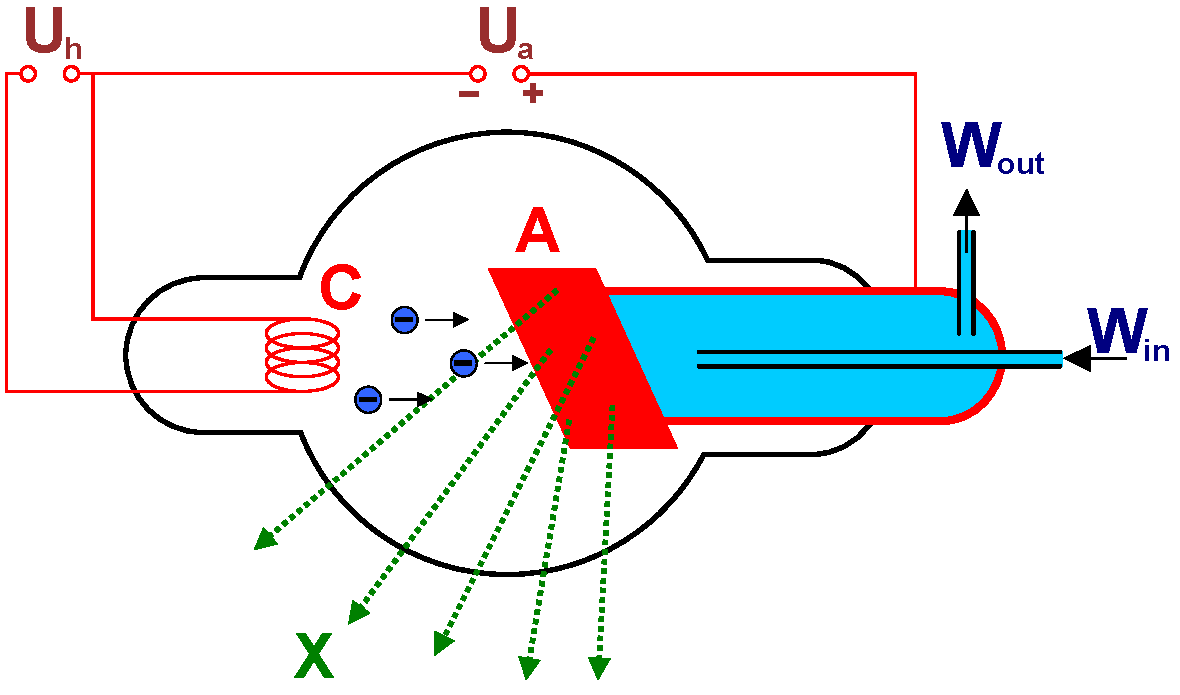
\includegraphics[width=0.5\textwidth]{Abbildungen/WaterCooledXrayTube.pdf}
    \caption{Schematischer Aufbau einer Röntgenröhre nach~\cite{Roentgenroehre}. Da beim Aufprall der Elektronen viel Wärme entsteht, muss die Anode mithilfe eines Wasserzuflusses $W_\text{in}$ gekühlt werden.}
    \label{fig:Roentgenroehre}
\end{figure}\\
Beim Aufschlagen auf die Anode werden die Elektronen abgebremst und strahlen Energie in Form von elektromagnetischen Wellen ab. Idealerweise würde die gesamte kinetische Energie in Röntgenstrahlung umgewandelt werden.
\begin{align}
  e U = E_\text{kin} = h \cdot \nu_\text{max} = \frac{hc}{\lambda_\text{min}}
\end{align}
Allerdings wird ein großer Teil der kinetischen Energie in Wärme umgesetzt, sodass die Anode gekühlt werden muss. Der schematische Aufbau einer Röntgenröhre ist in Abbildung~\ref{fig:Roentgenroehre} dargestellt.\\
Das Emissionsspektrum der Anode wird durch ihr Material und der Beschleunigungsspannung der Röntgenröhre bestimmt und setzt sich aus zwei Komponenten zusammen.\\
Die erste Komponente wird \glqq{}weiße Röntgenstrahlung\grqq{} genannt und erscheint allein durch das Abbremsen der Elektronen in der Oberflächenschicht des Targets. Die zweite Komponente bildet die charakteristische Röntgenstrahlung, die normalerweise aus zwei Linien besteht. Hier geschehen Übergänge zwischen den inneren Schalen der Atome des Targets. Gewöhnlich sind die Schalen vollständig mit Elektronen besetzt, jedoch können die hochenergetischen, eingeschossenen Elektronen die gebundenen Elektronen herausschlagen und dort freie Energieniveaus erzeugen. In diese können anschließend Elektronen höherer Niveaus unter Photonenemission übergehen. Diese Linien fester Frequenz werden im Spektrum als K$_\alpha$- bzw. als K$_\beta$-Linien bezeichnet (siehe Abbildung~\ref{fig:Roentgenspektrum}). Das 'K' steht für die Schale, die besetzt wird und der Index beschreibt, aus welcher Schale das Elektron kam, welches den Platz besetzt. Für $\alpha$ handelt es sich um die nächstliegende L-Schale.\vspace{-5mm}
\begin{figure}[htp]
    \centering
    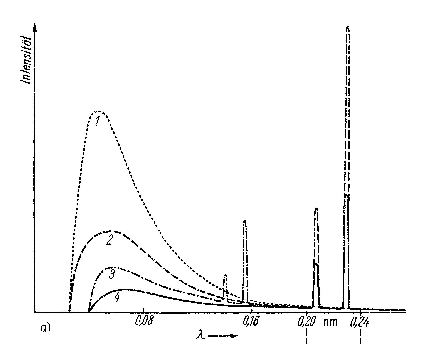
\includegraphics[width=0.5\textwidth]{Abbildungen/Roentgenspektrum.pdf}
    \caption{Brems- und charakteristisches Spektrum von Röntgenröhren mit verschiedenem Anodenmaterial. Bei der größten Emissionslinie handelt es sich um die K$_\alpha$-Linien. Bei $\lambda =\SI{0,21}{\nano\metre}$ befinden sich die K$_\beta$-Linien.~\cite[S.361]{Kleber}}
    \label{fig:Roentgenspektrum}
\end{figure}\\
Damit sich aus dem breiten Spektrum einer Röntgenröhre eine möglichst monochromatische Linie ergibt, wird meist ein Filter verwendet, um die weiße Bremssstrahlung und höhere charakteristische Linien wie K$_\beta$ auszublenden. Hierbei wird ausgenutzt, dass bei dem Durchgang durch ein Medium die Röntgenstrahlung zum Teil absorbiert nach einem Exponentialgesetz absorbiert wird.
\begin{align}
  I = I_0 \exp(-\mu d)
\end{align}
Hierbei bezeichnet $I$ die Intensität nach dem Durchdringen der Schicht der Dicke $d$ mit dem Absorptionskoeffizienten $\mu$. Das Absorptionsspektrum der Elemente weißt eine Kantenstruktur auf. Die $K_\beta$-Strahlung eines Elements der Ordnungszahl $Z$ kann durch den Einsatz eines Absorptionsfilters bestehend aus einem Element mit $Z-1$ eliminiert werden, da sich Absorptionskante und K$_\beta$-Linie überdecken. Das im Versuch verwendete Target ist Kupfer, weshalb sich ein Absorptionsfilter aus Nickel anbietet.

\subsection{Kristallographie}
Festkörper lassen sich in verschiedene Klassen einteilen. Ein spezielles Kriterium stellt ihre räumliche Struktur dar. Dabei wird unterschieden zwischen Einkristallen, polykristallinen Festkörpern, amorphen Festkörpern und Flüssigkristallen~\cite{Demtroeder}. Im Folgenden wird sich auf die Einkristalle beschränkt, bei denen die Orte der Atome durch ein periodisches Gitter von Raumpunkten beschreibbar ist. Für ideale Einkristalle erstreckt sich das periodische Gitter über den gesamten Kristall. Dies wird Fernordnung genannt.\\
Für die analytische Beschreibung wird dem Gitter ein Koordinatensystem zugrunde gelegt. Der Nullpunkt wird in einen beliebigen Gitterpunkt gesetzt und die Ortsvektoren $\bm{a}, \bm{b}, \bm{c}$ zu den drei Nachbarpunkten stellen die Basis des Gitters dar. Die Beträge der Vektoren $a_0, b_0, c_0$ und die entsprechenden Winkel zwischen den Vektoren $\alpha, \beta, \gamma$ werden als Gitterkonstanten bezeichnet. Das Parallelipiped, welches sich aus den drei Basisvektoren aufbaut, wird Elementarzelle genannt. Lässt sich das gesamte Gitter, durch Translationen einer Elementarzelle aufbauen,
\begin{align}
  \bm{R} = \sum_{i=1}^3 n_i \cdot \bm{a}_i \qquad \text{mit}\quad n_i \in \mathbb{Z}
\end{align}
so wird es auch Translationsgitter genannt~\cite{Demtroeder}. Da die Wahl der Elementarzelle nicht eindeutig ist, werden die Achsen des Gitters so gewählt, dass die Translationen möglichst \textit{kurz} sind. Unter dieser Voraussetzung lassen sich alle Einkristalle in sieben verschiedene Achsensysteme einteilen:
\begin{table}[ht]
	\centering
	\caption{Einteilung der Einkristalle in Achsensystem nach~\cite{Kleber}.}
	\label{tab:Achsensysteme}
	\begin{tabular}{l l l l}
		\toprule
	   Gitterart & Gittervektoren & Gitterwinkel\\
	 	\midrule
			Triklin & $a_0 \neq b_0 \neq c_0 \neq a_0$ & $\alpha \neq \beta \neq \gamma\neq \alpha$\\
			Monoklin & $a_0 \neq b_0 \neq c_0 \neq a_0$ & $\alpha = \beta = 90^\circ, \gamma\neq 90^\circ$\\
      Rhombisch & $a_0 \neq b_0 \neq c_0 \neq a_0$ & $\alpha = \beta =\gamma =90^\circ$\\
      Hexagonal & $a_0 = b_0 \neq c_0$ & $\alpha = \beta = 90^\circ, \gamma = 120^\circ$\\
      Rhombobedrisch & $a_0 = b_0 = c_0$ & $\alpha = \beta =\gamma \neq 90^\circ$\\
      Tetragonal & $a_0 = b_0 \neq c_0$ & $\alpha = \beta =\gamma =90^\circ$\\
      Kubisch & $a_0 = b_0 = c_0$ & $\alpha = \beta =\gamma =90^\circ$\\
	\end{tabular}
\end{table}\\
% \begin{enumerate}
%   \item Triklin: $a_0 \neq b_0 \neq c_0 \neq a_0, \quad \alpha \neq \beta \neq \gamma\neq \alpha$
%   \item Monoklin: $a_0 \neq b_0 \neq c_0 \neq a_0, \quad \alpha = \beta = 90^\circ, \gamma\neq 90^\circ$
%   \item Rhombisch: $a_0 \neq b_0 \neq c_0 \neq a_0, \quad \alpha = \beta = \gamma = 90^\circ$
%   \item Hexagonal: $a_0 = b_0 \neq c_0, \quad \alpha = \beta = 90^\circ, \gamma = 120^\circ$
%   \item Rhombobedrisch: $a_0 = b_0 = c_0, \quad \alpha = \beta =\gamma \neq 90^\circ$
%   \item Tetragonal: $a_0 = b_0 \neq c_0, \quad \alpha = \beta =\gamma = 90^\circ$
%   \item Kubisch: $a_0 = b_0 = c_0, \quad \alpha = \beta =\gamma =90^\circ$
% \end{enumerate}
Werden diese Achsensysteme den möglichen Translationsgittern zugrunde gelegt, ergeben sich 14 Elementarzellen oder \textit{\textsc{Bravais}-Gitter}.\\
Im Rahmen des Versuchs werden nur die Kubischen Gitter betrachtet, woraus folgt, dass nur eine Gitterkonstante ermittelt werden muss.
\begin{align}
  a_0 = b_0 = c_0 =: a_0
\end{align}

\subsubsection{Millersche Indizes und Netzebenen}
Eine Möglichkeit zur Beschreibung einer Kristallfläche ist ihren Bezug auf ein bestimmtes Achsensystem anzugeben. Durch drei Gitterpunkte wird eine \textit{Netzebene} definiert. Die relative Ordnung wird durch die Schnittpunkte mit den Achsen festgelegt. Haben die Schnittpunkte die Form
\begin{align}
  S_1 = m_1 \bm{a} \qquad S_2 = m_2 \bm{b} \qquad S_3 = m_3 \bm{c},
\end{align}
dann bilden die reziproken Werte multipliziert mit einer kleinsten ganzen Zahl $p$, welche die Kehrwerte zu teilerfremden ganzen Zahlen macht, die \textit{\textsc{Miller}'schen Indizes}.
\begin{align}
  h = \frac{p}{m_1} \qquad k = \frac{p}{m_2} \qquad l = \frac{p}{m_3}
\end{align}
Jedes Tripel (hkl) definiert eine Schar paralleler Netzebenen. Die Richtung der Ebenen wird durch die Ebenennormale $\bm{n} = (h,k,l)$ bestimmt.

\subsubsection{Laue-Gleichungen und Bragg'sche Bedingung}
Treffen Röntgenstrahlen auf ein Elektron auf, wird dieses in Schwingung versetzt und oszilliert in Phase mit der Röntgenwelle und stellt ebenso eine Quelle von Kugelwellen dar, die miteinander interferieren. Wird ein Atom von der Röntgenwelle getroffen, so streut das gesamte Elektronen-Ensemble.\\
Die Beugung an einem Kristallgitter kann analog zur Begung an einem eindimensionalen Punktgitter betrachtet werden. Für einen Einfallswinkel $\varphi_0$ paralleler Röntgenstrahlen auf das Gitter, die unter dem Winkel $\varphi$ gebeugt wird ergibt sich aus der Forderung für konstruktiver Interferenz bei einem Gangunterschied von einem Vielfachen der Wellenlänge folgende Bedingung
\begin{align}
  a_0 (\cos(\varphi) - \cos(\varphi_0)) = h\,\lambda.\label{eqn:Laue1}
\end{align}
Da sich die Elementarzelle aus drei Punktgittern entlang der gewählten Koordinatenachsen aufbaut, ergeben sich aus \eqref{eqn:Laue1} die \textit{\textsc{Laue}-Gleichungen}
\begin{align}\label{eqn:Laue2}
  a_0 (\cos(\varphi_a) - \cos(\varphi_{a0})) &= h\,\lambda\notag\\
  b_0 (\cos(\varphi_b) - \cos(\varphi_{b0})) &= k\,\lambda\\
  c_0 (\cos(\varphi_c) - \cos(\varphi_{c0})) &= l\,\lambda\notag.
\end{align}
Die \textsc{Laue}-Indizes $(hkl)$ stellen dabei die mit der Beugungsordnung $n$ multiplizierten \textsc{Miller}-Indizes dar.
Eine zu den \textsc{Laue}-Gleichung äquivalente Bedingung ergibt sich, wenn die Beugung der Röntgenstrahlen als eine Reflexion an den Netzebenen des Gitters gedeutet wird.  Dies führt zur \textit{Bragg-Bedingung}
\begin{align}
  n\cdot \lambda = 2d\cdot \sin(\vartheta),
\end{align}
wobei $\theta$ den Einfalls- und Reflexionswinkel an der Netzebenenschar beschreibt (siehe Abbildung~\ref{fig:Roentgenbeugung}).
\begin{figure}[htp]
    \centering
    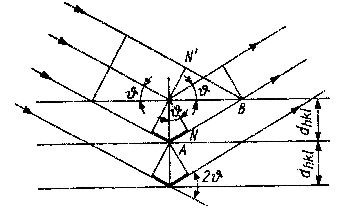
\includegraphics[width=0.3\textwidth]{Abbildungen/Roentgenbeugung.pdf}
    \caption{Beugung eines Röntgenstrahlbündels an einer Netzebenenschar mit Abstand $d_{hkl}$.~\cite[S.367]{Kleber}}
    \label{fig:Roentgenbeugung}
\end{figure}\\
Der Abstand $d$ einer Netzebenschar parallel zum Normalenvektor $\bm{n}=(h,k,l)$ ist abhängig von den Laue-Indizes und den Dimensionen der Elementarzelle und nimmt folgende Form an:
\begin{align}
  d_{hkl} = \frac{1}{\sqrt{\left(\frac{h}{a_0}\right)^2+\left(\frac{k}{b_0}\right)^2+\left(\frac{l}{c_0}\right)^2}}\label{eqn:Ebenabstand}
\end{align}
Für die im Versuch betrachteten kubischen Kristallgitter vereinfacht sich \eqref{eqn:Ebenabstand} zu
\begin{align}
  d_{hkl} = \frac{a_0}{\sqrt{h^2+k^2+l^2}}
\end{align}

\subsection{Das Debye-Scherrer Verfahren}
\begin{figure}[htp]
    \centering
    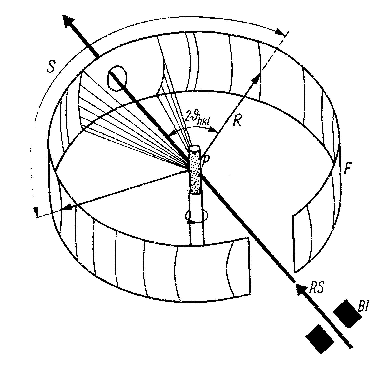
\includegraphics[width=0.3\textwidth]{Abbildungen/Debye-Sherrer-Kamera.pdf}
    \caption{Strahlenverlauf beim Debye-Scherrer-Verfahren.~\cite[S.375]{Kleber}}
    \label{fig:Debye-Kamera}
\end{figure}\\

% ***** Zwei Bilder nebeneinander *****

% \begin{figure}[htp]
%     \centering
%     \begin{subfigure}{0.45\textwidth}
%         \includegraphics[width=\textwidth]{Bilder/Beispielbild.png}
%     \end{subfigure}
%     \begin{subfigure}{0.45\textwidth}
%         \includegraphics[width=\textwidth]{Bilder/Beispielbild.png}
%     \end{subfigure}
%     \caption{Beschreibung}
% \end{figure}

%***** Tabellen *****
% \begin{table}[ht]
% 	\centering
% 	\caption{Überschrift der Tabelle}
% 	\label{tab:Tabelle1}
% 	\begin{tabular}{l c c c}
% 		\toprule
% 	    text & text & text & text\\
% 	 	\midrule
% 			text & text & text & text\\
% 			text & text & text & text
% 	\end{tabular}
% \end{table}

% *********************************************
% ***** KAPITEL 3 *****************************
% *********************************************
\section{Versuchsdurchführung} \label{sec:Versuchsdurchführung}
Für die Aufnahme der zwei Diffraktogramme wurde die kristalline Substanz zunächst mithilfe eines Mörser zu einem kleinen Pulver zerkleinert. Anschließend wurde eine kleine Menge des Pulvers in eine \SI{0.1}{\milli\metre} große Glaskapillare eingefüllt und diese mit einem Klebwachs an der Drehachse der \textsc{Debye\--Sherrer}\--Kamera befestigt. Dabei wurde darauf geachtet, dass die Glaskapillare möglichst senkrecht aufgebracht ist und die Drechachse mittig ausgerichtet ist. Die Justage erfolgte mithilfe eine Justierlupe durchgeführt.
\subsection{Aufnahme der Beugungsbilder}
In der Dunkelkammer wurde unter Rotlicht der Röntgenfilm in die Kamera eingelegt, sowie Primärstrahlfänger und Blende wieder eingesetzt. Beim Einlegen des Films wurde mit einer Schere die untere rechte Ecke des Films abgeschnitten, um die Orientierung des Films innerhalb der Kamera später rekonstruieren zu können.\\
Im weiteren Verlauf wurde die \textsc{Debye\--Sherrer}\--Kamera auf die entsprechende Halterung in der Röntgenkamera gesetzt und der Motor zur Drehung des Präparats montiert.\\
Für die Aufnahmen wurde eine Hochspannung von \SI{35}{\kilo\volt} mit einem Anodenstrom von \SI{30}{\milli\ampere} eingestellt. Die erste Probe wurde ohne Filter 10 Minuten lang beleuchtet.\\
Für die zweite Probe wurde ein Nickel-Filter eingesetzt und insgesamt 30 Minuten lang beleuchtet.
\subsection{Entwicklung des Röntgenfilms}
Nach der Beleuchtung der Probe wurde der Röntgenfilm in der Dunkelkammer aus der Kamera herausgeholt und entwickelt. Dafür wurde der Film für 4 Minuten in das Entwicklerbad getaucht. Dabei wurde der Film immer wieder leicht bewegt, um eine gleichmäßige Wirkung der Entwicklersubstanz zu gewährleisten.\\
Anschließend wurde der Film kurz in einem Wasserbad gewässert und anschließend für 15 Minuten in ein Fixierbad getaucht. Zuletzt wurde der Film erneut für weitere 20 Minuten in das Wasserbad gebracht und im Anschluss noch mit Netzmittel behandelt.


% *********************************************
% ***** KAPITEL 4 *****************************
% *********************************************
\section{Ergebnisse und Diskussion}
Tabellen mit gemessenen und berechneten Werten, Abbildungen, Diagramme usw. mit Unterschriften sowie Vorgehensweise, Kommentare, Fehlerrechnung.\\
Diskussion der Messergebnisse, Diagramme, Fehlerquellen usw. aus physikalischer Sicht, Vergleich mit der Literatur und theoretischen Werten usw.

% *********************************************
% ***** KAPITEL 4 *****************************
% *********************************************
\section{Zusammenfassung}
Lorem ipsum dolor sit amet, consetetur sadipscing elitr, sed diam nonumy eirmod tempor invidunt ut labore et dolore magna aliquyam erat, sed diam voluptua. At vero eos et accusam et justo duo dolores et ea rebum. Stet clita kasd gubergren, no sea takimata sanctus est Lorem ipsum dolor sit amet. Lorem ipsum dolor sit amet, consetetur sadipscing elitr, sed diam nonumy eirmod tempor invidunt ut labore et dolore magna aliquyam erat, sed diam voluptua. At vero eos et accusam et justo duo dolores et ea rebum. Stet clita kasd gubergren, no sea takimata sanctus est Lorem ipsum dolor sit amet.

% ***** Literaturverzeichnis ******************

\begin{thebibliography}{xxx}
	\bibitem{Demtroeder}
	W. Demtröder: \textit{Experimentalphysik}. Springer Verlag Berlin Heidelberg New York 2008 (5. Auflage).
	\bibitem{Glockner}
	R. Glocker: \textit{Materialprüfung mit Röntgenstrahlen}. Springer Verlag Berlin Heidelberg New York 1985.
  \bibitem{Kleber}
	W. Kleber u.a.: \textit{Einführung in die Kristallographie}. Oldenbourg Wissenschaftsverlage 2010 (19. Auflage).
  \bibitem{Roentgenroehre}
  Aufbau einer Röntgenröhre: \url{wikimedia.org/wiki/File:WaterCooledXrayTube.svg}. Stand: 20.10.2019
\end{thebibliography}

\end{document}
